\section{はじめに}

\subsection{アロステリー}
タンパク質のアロステリー現象は、
リガンド結合や外部刺激によって生じる構造変化が刺激受容部位から遠隔の活性部位に影響を及ぼす現象であり、
そのメカニズム解明は生命現象の理解と創薬研究の中心的的題の一つである。
%参考文献:アロステリーの特性
%2009「アロステリーと協同性の再考」
%https://onlinelibrary.wiley.com/doi/10.1110/ps.03259908
アロステリーはタンパク質の機能を制御する重要な特性であり\cite{Cui2009}、
リガンド結合など外部刺激のシグナルが残基間相互作用を介してサブ\,\text{\AA}~数十\,\text{\AA}離れた活性部位に伝達する仕組みを提供する。

\subsection{グラフ理論}
アロステリーの離れた場所間のコミュニケーションを解明する一つの方法として、
グラフ理論\cite{Zhou2018}を用いたアプローチが注目されている。
グラフ理論は、分子内の残基間の相互作用をネットワークとして表現し、
複雑な動的挙動を解析するための強力なツールとして広く利用されてきた\cite{Doncheva2011}\cite{Martin2011}\cite{Doncheva2012}。
%参考文献:グラフ理論
%2011「タンパク質構造の残基ネットワークの解析と可視化」
%https://www.cell.com/trends/biochemical-sciences/abstract/S0968-0004(11)00013-2?_returnURL=https%3A%2F%2Flinkinghub.elsevier.com%2Fretrieve%2Fpii%2FS0968000411000132%3Fshowall%3Dtrue
%2011「RING: タンパク質構造における相互作用残基、進化情報、エネルギーのネットワーク化」
%https://academic.oup.com/bioinformatics/article/27/14/2003/193801?login=false
%2012「生物学的ネットワークとタンパク質構造のトポロジー解析とインタラクティブな可視化」
%https://www.nature.com/articles/nprot.2012.004
グラフ理論では、タンパク質のアミノ酸残基の相互作用を、
ノードとエッジを用いたアミノ酸ネットワークとして表すことができる。
\begin{itemize}
  \item \textbf{ノード}:アミノ酸残基(原子やタンパク質全体も可能)
  \item \textbf{エッジ}:ノード同士の相互作用
\end{itemize}

そしてエッジに重みづけをすることで、エッジを同じ距離1とするのではなく、
各結合ごとに強度を振り分けることが可能である。

タンパク質間の相互作用ネットワークをグラフとしてモデル化することで、
シグナル伝達機構を解釈しやすくなり、生命現象の解明や新薬の開発に役立っている。
そのようなモデルは、ネットワーク内の最短経路の存在の重要性を強調\cite{Ghosh2007}しており、
それらが離れた部位間での効率的な情報伝達に寄与していることを示している。
%参考文献:最短経路
%2007「分子動力学シミュレーションと構造ネットワーク解析によるメチオニルtRNA合成酵素のコミュニケーション経路の研究
%https://www.pnas.org/doi/full/10.1073/pnas.0704459104
また、その前提のもとで、
高い中心性を持つ残基\cite{amitai2004}やネットワーク上における最短経路上によく現れる残基\cite{delsol2006}を解析することで、
機能的残基を同定してきた。
%参考文献:中心性
%2004「タンパク質構造のネットワーク解析により機能残基を特定」
%https://www.sciencedirect.com/science/article/pii/S0022283604013592
%参考文献:最短経路
%2006「ネットワーク通信における短い経路を維持するために重要な残基がタンパク質のシグナル伝達を媒介する」
%https://www.embopress.org/doi/full/10.1038/msb4100063
実際にこれらの残基はタンパク質の折りたたみにおける重要なアミノ酸や酵素ファミリーの活性部位残基であると関連付けられている。

\subsection{本研究の位置づけ}
ここまで、シグナルはある「経路」に沿って伝達するという仮説に基づいた解析について述べてきた。
しかし、単純な「最短経路モデル」だけでは、アロステリーの情報伝達を十分に説明できない可能性がある。
ピコ秒オーダーの残基間エネルギー移動過程\cite{Lim1996}とミリ秒以上のアロステリック遷移\cite{Changeux2005}の時間スケールの違いを考慮すると、
リガンド結合部位から活性部位まで情報が伝言ゲームのように最短経路上を通ると考えるにはあまりに単純すぎるのではないかと考えられるからだ。
%参考文献:アロステリー、時間スケールと空間スケール
%2005「シグナル伝達のアロステリック機構」
%https://www.science.org/doi/abs/10.1126/science.1108595
%大きな謎
%2008「アロステリー:「生命の第二の秘密」の図解による定義」
%https://www.sciencedirect.com/science/article/pii/S0968000408001643
%参考文献:グラフ理論
%https://pubs.acs.org/doi/10.1021/acs.chemrev.7b00305

実際にアロステリーは特定の結合が経路を介して直接的に伝播するメカニズムなのではなく、
タンパク質全体の構造分布の再編成によって引き起こされる、
つまりアロステリーは特定のエネルギー伝達の経路を必要としないと言及する先行研究\cite{Hilser2007}\cite{Pan2000}が存在する。
つまりこのモデルは再考の必要がある。
%アンサンブルアロステリー
%https://www.pnas.org/doi/10.1073/pnas.0700329104

そうしたことを踏まえて、T. Ishikura, Y. Iwata, T. Hatano, T. Yamato は、
アミノ酸間のエネルギーのやりとりの強弱をエネルギー交換ネットワークとして表現するEnergy Exchange Network Model(EENモデル)を確立\cite{Ishikura2015}した。
このモデルを適用してPDZドメインのC末端の$\alpha$ヘリックスの除去前後で比較すると、
$\alpha$ヘリックスがリガンド結合部位と他の領域のつながりを保つ役割を果たしていたことが明らかになり、
これは$\alpha$ヘリックスの除去がリガンド親和性を21倍減少させる先行研究の見解と一致していた。
つまりEENの変化と機能の変化を結びつける画期的なモデルであることが証明された。

%EEN
%https://onlinelibrary.wiley.com/doi/abs/10.1002/jcc.23989

そこで本研究では、EENモデルでも使用している「ネットワークの再編」の概念をベースにし、
$\beta_2$アドレナリン受容体($\beta_2$AR)という膜タンパク質の活性化によるネットワークの再編を比較することで、
$\beta_2$ARのシグナル伝達機構を解析することを目的とする。

EENモデルでは「残基」レベルのコミュニケーションに着目していたが、
本研究では「コミュニティ(残基集団)」レベルの中間的スケールでの再編成に着目する。
アロステリーのタンパク質全体というグローバルな動的性質と、残基や原子の相互作用という局所的な動的性質の両方を効果的に取り入れることができるからだ。

シグナルはドミノ倒しのように残基間の明確に定義された特定の経路を伝播しているのではないかというのは直感的に考えつくことなので多くの研究があるが、
残基間のエネルギー移動過程はピコ秒程度のため、この過程だと数10ピコ秒で伝わってしまうことになる。
そうではなく、活性化によってコミュニティという中間的スケールの残基集団の時間のかかる再編によって、
シグナルを伝達させているのではないかと推測した。

実際に$\beta_2$ARは、同じファミリーに属するバクテリアロドプシン(bR)やロドプシン(Rho)と違い光励起がないため、
エネルギーを効果的に散逸させる進化的必要性がない\cite{Helmer2022}という背景からも、
この仮説を裏付けることができる。

\section{$\beta_2$アドレナリン受容体($\beta_2$AR)}
\label{sec:b2ar}

\subsection{基本情報}
$\beta_2$アドレナリン受容体($\beta_2$AR)は、Gタンパク質共役受容体(GPCR)の一種である。
GPCRは細胞膜に存在する膜タンパク質であり、ホルモンや神経伝達物質などの細胞外刺激を認識し、それを細胞内のシグナルに変換する役割を担っている。
また、視覚、嗅覚、味覚といった感覚にも関与し、生体内の多様なシグナル伝達経路において中心的な役割を果たしている。

GPCRは7回膜貫通構造を持つことが特徴であり、各膜貫通ヘリックス(TM1からTM7)は、細胞外ループ(ECL)と細胞内ループ(ICL)を介して他のヘリックスと連結されている。
この構造により、細胞外でのリガンド認識と細胞内でのシグナル伝達を効率的に行うことが可能となる。

%TM1-7
\begin{figure}[htbp]
  \centering
  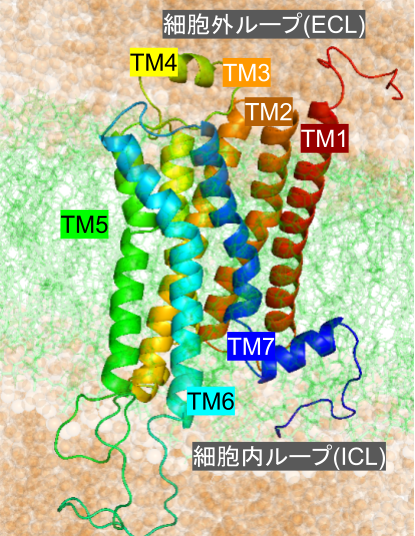
\includegraphics[width=0.8\textwidth]{system-all-with-TM.png}
  \caption{$\beta_2$ARの膜貫通ヘリックス。}
  \label{fig:all}
\end{figure}

\newpage

膜タンパク質の構造データはProtein Data Bank(PDB)から取得し、
$\beta_2$ARの不活性状態として2RH1\cite{cherezov2007},活性状態として3P0G\cite{rasmussen2011}を用いる。
%2RH1の構造情報2007
%https://www.science.org/doi/10.1126/science.1150577
%3P0Gの構造情報2011
%https://www.nature.com/articles/nature09648

\subsection{活性化に伴う構造的変化}
$\beta_2$ARのinactive状態からactive状態への活性化は、
リガンド結合部位に結合したアゴニストによって引き起こされる。
すると受容体が活性化され、膜貫通ヘリックスの動的な再配置により、細胞内でGタンパク質結合部位を露出させる。
すると細胞内シグナルが伝達し、特にGsといったGタンパク質の結合が促進される。
Gsはヘテロ三量体型タンパク質であり、その活性化により細胞内でアデニル酸シクラーゼが刺激され、cAMP(サイクリックAMP)の産生が増加する。
この過程\cite{philip2007}を通じて信号が増幅し、細胞内応答を引き起こす。
%参考文献:GPCRのシグナル伝達機構
%2007「G タンパク質共役受容体とそれに対応する G タンパク質を介したシグナル伝達は、化学量論的に制限されたモデルに従う」
%https://www.sciencedirect.com/science/article/pii/S002192582087389X

%詳細の構造と、リガンド・gタンパク質結合部位を示す
$\beta_2$ARのリガンド結合部位は膜貫通ヘリックス(TM)の間に位置し、細胞外の刺激を感知する。
一方で、Gタンパク質との結合は細胞内ループおよび細胞質側ドメインを介して行われる。


\subsection{モチーフ}
$\beta_2$ARの活性化において、特定のモチーフ\cite{nygaard2009ligand}\cite{lee2013mapping}
が重要な役割を果たしていることが知られている。

%参考文献:モチーフ
%2009「7TM受容体構造におけるリガンド結合とマイクロスイッチ」
%https://www.sciencedirect.com/science/article/pii/S0165614709000546
%参考文献:モチーフ
%2013「Gタンパク質共役受容体の分子内シグナル伝達のマッピング」
%https://onlinelibrary.wiley.com/doi/10.1002/prot.24451
%参考文献:保存水
%2009「保存された水はファミリーA(ロドプシン様)Gタンパク質共役受容体の構造的および機能的活性化を媒介する」
%https://www.pnas.org/doi/10.1073/pnas.0903545106
モチーフとは、タンパク質中の特定の機能に関連する保存されたアミノ酸配列のことであり、GPCRではアロステリックシグナル伝達やコンフォメーション変化を介して受容体の機能を調節する。
$\beta_2$ARを含むクラスA GPCRでは、以下の4つの主要な保存モチーフ(DRY、CWxP、NPxxY、PIF)と「イオンロック」が重要な役割を果たしている。

\begin{itemize}
  \item \textbf{DRYモチーフ}  
  TM3の細胞質側領域に位置し、Asp(D)-Arg(R)-Tyr(Y)から構成される。inactive状態ではTM6のGluとイオンロックを形成し、構造を安定化させている。一方、active状態ではイオンロックが解除され、Gタンパク質との結合が可能になる。

  \item \textbf{CWxPモチーフ}  
  TM6のリガンド結合ポケットの底部に位置し、Cys(C)-Trp(W)-任意の残基(x)-Pro(P)から構成される。inactive状態ではTrpがリガンド結合ポケットを開いた状態を維持しているが、active状態ではTrpが「トグルスイッチ」として機能し、ポケットを閉じる役割を果たす。

  \item \textbf{NPxxYモチーフ}  
  TM7の細胞質側に位置し、Asn(N)-Pro(P)-任意の残基(xx)-Tyr(Y)から構成される。このモチーフにおけるTyrは、不活性状態と活性状態で異なる立体配座間を回転することで、構造の変化を媒介する。

  \item \textbf{PIFモチーフ}  
  TM4、TM5、TM6にまたがる位置に存在し、Pro(P)-Ile(I)-Phe(F)から構成される。このモチーフにおけるPheはスイッチとして機能し、活性化時に異なる立体配座間で方向を変えることで重要な役割を果たす。

  \item \textbf{イオンロック}  
  TM3とTM6の間に位置している。不活性状態ではイオンロックが形成され、構造を安定化させているが、活性化時にはこのロックが解除され、GPCRの完全な活性化を促進する。
\end{itemize}

\subsection{保存された結晶水}
%水はアミノ酸と同じくらい重要だと説明
また水分子も、生物学的システムにおいて重要な役割を果たすことが知られており、特にGPCRの活性化メカニズムにも深く関与している。
脂質二重層の誘電率は2から5程度であり水(一般的に誘電率80程度)と比べると非常に低いため、
クーロンの法則に基づき、電荷間の静電相互作用が水環境に比べてはるかに強くなる。
すると脂質環境下では荷電残基が重要な役割を果たしており、それが極性持つ近傍の水やイオンと強く相互作用する。

実際にロドプシンをはじめとするGPCRで高度に保存された水は、活性化過程においてアロステリックを仲介する機能を果たすことが示されている\cite{angel2009conserved}。
$\beta_2$ARにおいても、膜貫通ドメイン内にはいくつかの保存された水分子が確認され、これらの水分子はアロステリックシグナル伝達に関与していると考えられる。
これらの水分子はアミノ酸残基と同じくらい受容体機能に重要であることが示されている。

そこで本研究でも、保存された結晶水をアミノ酸残基と同等の扱いとして露に取り入れることで、
タンパク質の実際の挙動をより忠実に表現することを可能にした。
